\documentclass[12pt,letterpaper]{article}

\usepackage{tikz}
\usetikzlibrary{shapes}

\usepackage{amssymb,amsmath,amsthm}
\usepackage{enumerate}
\usepackage[margin=1.25in]{geometry}
\usepackage{graphicx,ctable,booktabs}
\usepackage{fancyhdr}
\usepackage[utf8]{inputenc}

\makeatletter
\newenvironment{problem}{\@startsection
       {section}
       {1}
       {-.2em}
       {-3.5ex plus -1ex minus -.2ex}
       {2.3ex plus .2ex}
       {\pagebreak[3]
       \large\bf\noindent{Problem }
       }
       }
\makeatother

\title{Parity \& Divisibility}
\author{Name: \underline{\hspace{5cm}}}
\date{February 7, 2015}

\pagestyle{fancy}
\lhead{Parity \& Divisibility}
\chead{} 
\rhead{\thepage} 
\lfoot{\small\scshape Grade 4 Olympic Math} 
\cfoot{} 
\rfoot{} 
\renewcommand{\headrulewidth}{.3pt} 
\renewcommand{\footrulewidth}{.3pt}
\setlength\voffset{-0.25in}
\setlength\textheight{648pt}
\setlength\headheight{15pt}

\begin{document}

\maketitle

\thispagestyle{empty}

\begin{problem}{Odd or even?}
For each of the following numbers, circle ``Odd'' or ``Even''.
\begin{enumerate}
 \item $17$ \hfill Odd \hspace{1em} Even
 \item $49494$ \hfill Odd \hspace{1em} Even
 \item $41 + 29 + 302$ \hfill Odd \hspace{1em} Even
 \item $621203 - 192935$ \hfill Odd \hspace{1em} Even
 \item $621203 \times 192935$ \hfill Odd \hspace{1em} Even
 \item $41 \times 29 \times 302$ \hfill Odd \hspace{1em} Even
\end{enumerate}
\end{problem}

\begin{problem}{Elementary School}
 At Applebury Elementary School, there is an even number of students,
 an odd number of teachers, and $17$ other staff members. Is the total
 number of people in this school even or odd? \hfill Answer: Odd \hspace{1em} Even
\end{problem}

\begin{problem}{Fair Share}
 Can I divide $21$ chocolates fairly among $2$ people? \hfill Answer: Yes \hspace{1em} No
 
 (I cannot cut any chocolates in half.)
\end{problem}

\begin{problem}{Even Number}
 All even numbers are divisible by $\underline{\hspace{2em}}$ and $\underline{\hspace{2em}}$.
\end{problem}

\begin{problem}{Rectangle}
 Look at the diagram below.
 
 \begin{center}
 \begin{tikzpicture}
  \draw[step=0.5] (0,0) grid (7,5.5);
 \end{tikzpicture}
 \end{center}
 
 \begin{enumerate}
  \item What are the dimensions of the rectangle? \hfill $\underline{\hspace{2em}}\times\underline{\hspace{2em}}$ 
  \item Is the number of small squares even or odd? \hfill Odd \hspace{1em} Even
  \item Is the number of small squares divisible by $3$? \hfill Yes \hspace{1em} No
  \item Is the number of small squares divisible by $11$? \hfill Yes \hspace{1em} No
 \end{enumerate}
\end{problem}

\begin{problem}{Divisibility}
 Are all of the following divisibility statements correct or incorrect? If incorrect,
 change the divisibility statement so that it becomes correct.
 
 \begin{enumerate}
  \item $6 \mid 2$
  \item $4 \mid 40$
  \item $3 \mid 99$
  \item $100 \mid 7801$
 \end{enumerate}

\end{problem}

\begin{problem}{Challenge}
 A ``cool'' number is a number that is divisible by all of $2$, $3$, $4$, and $6$.
 For example, $60$ is a cool number but $100$ is not (since it isn't divisble by $3$).
 Between $1$ and $1000$ (and including both $1$ and $1000$), how many numbers are cool?
\end{problem}



\end{document}